%%%%%%%%%%%%%%%%%%%%%%%%%%%%%%%%%%%%
% Alexander Powell
% CSCI 680 - Compiler Optimization
% Prof: Bin Ren
% Homework #1
% Due: 09.21.2016
%%%%%%%%%%%%%%%%%%%%%%%%%%%%%%%%%%%%

\documentclass[10pt]{article} %
\usepackage{fullpage}
\usepackage{graphicx}
\usepackage{graphics}
\usepackage{psfrag}
\usepackage{amsmath,amssymb}
\usepackage{enumerate}
\usepackage[final]{pdfpages}

\setlength{\textwidth}{6.5in}
\setlength{\textheight}{9in}

\newcommand{\cP}{\mathcal{P}}
\newcommand{\N}{\mathbb{N}}
\newcommand{\Z}{\mathbb{Z}}
\newcommand{\R}{\mathbb{R}}
\newcommand{\Q}{\mathbb{Q}}
\newcommand{\points}[1]{{\it (#1 Points)}}
\newcommand{\tpoints}[1]{{\bf #1 Total points.}}

\title{CSCI 680 -- Compiler Optimization \\
Homework 1 \\
{\large{\bf Due: September 21, 2016}}}
\date{}
\author{Alexander Powell}


\begin{document}
\maketitle
\begin{enumerate}

\item \textbf{Control Flow Analysis}

\begin{enumerate}[(a)]
\item 

Based on the line numbers of the given code, the set of basic blocks can be written as: 
$$ \{ \{ 1 \}, \{ 2, 3 \}, \{ 4, 5, 6 \}, \{ 7, 8 \} \}. $$

\item 

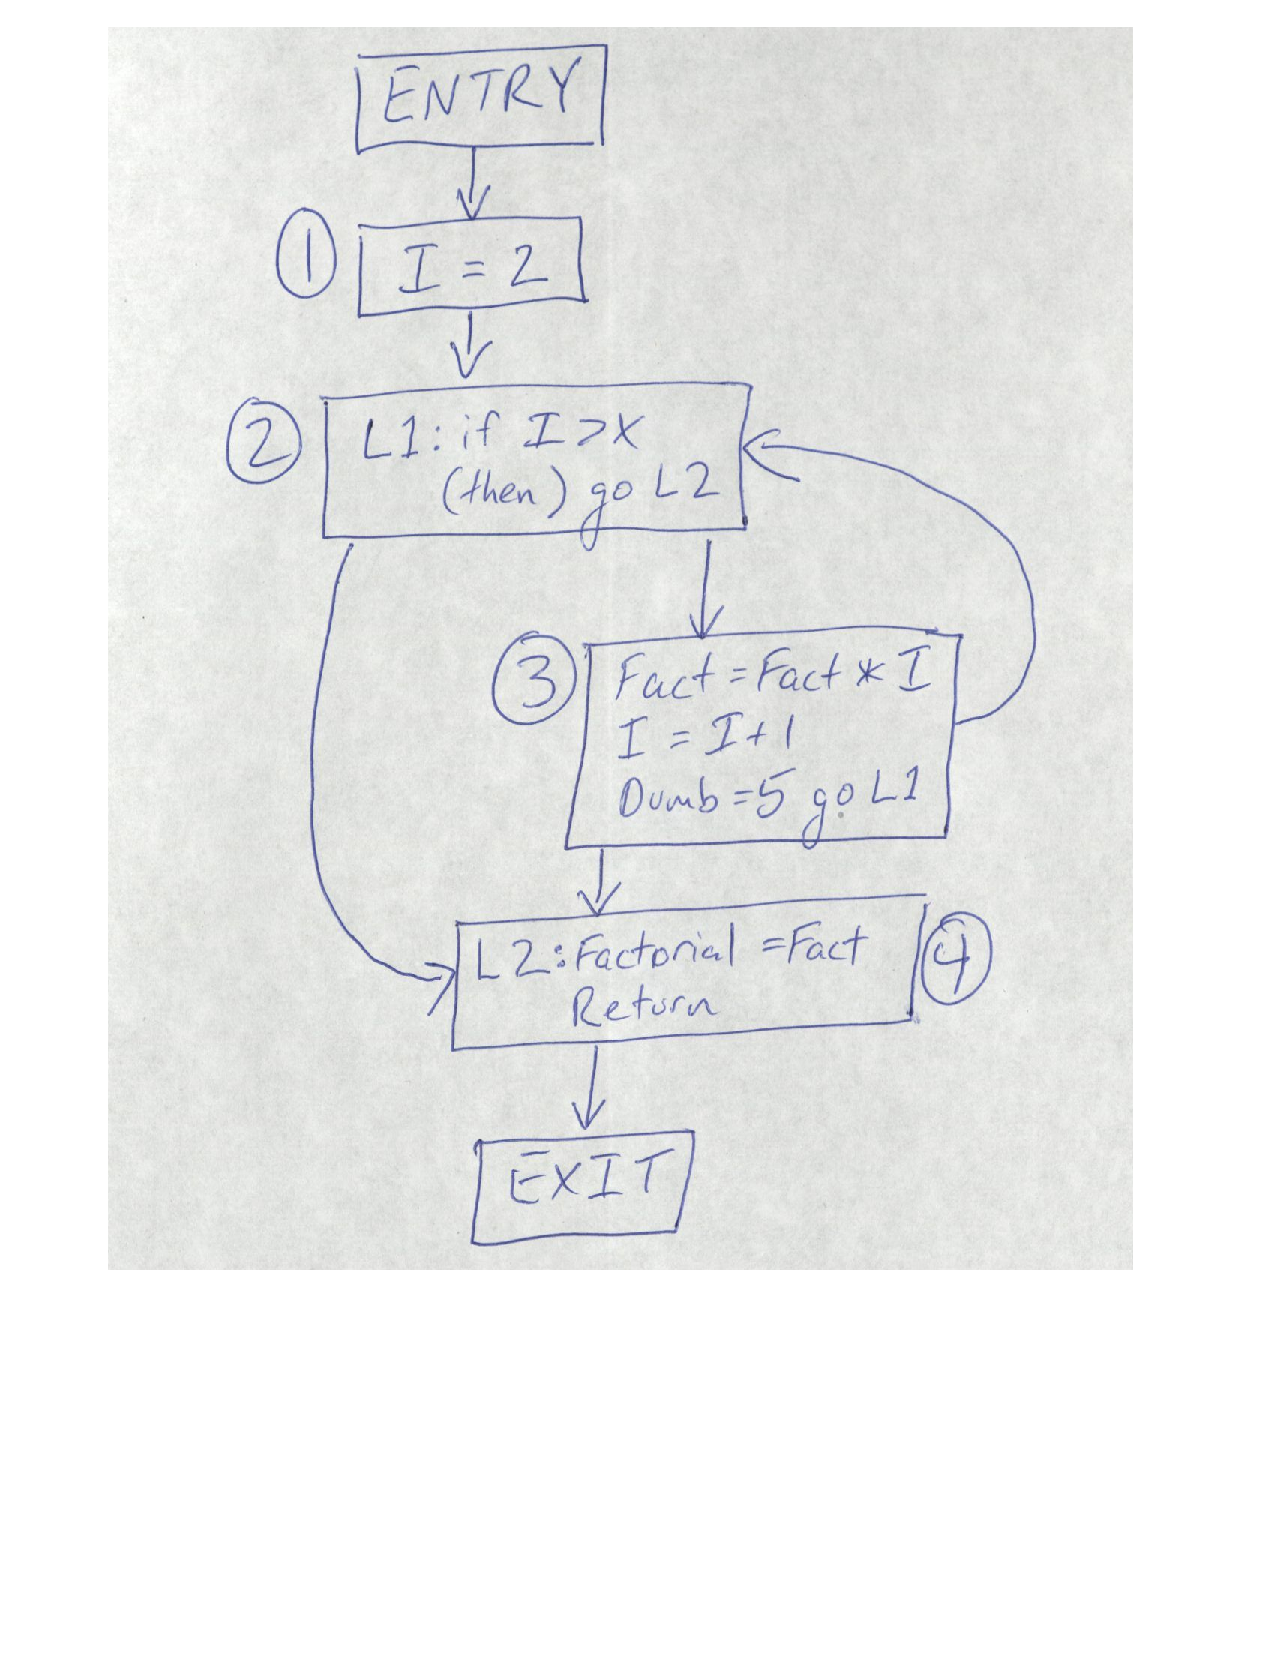
\includepdf[scale=0.25]{p1b.pdf}
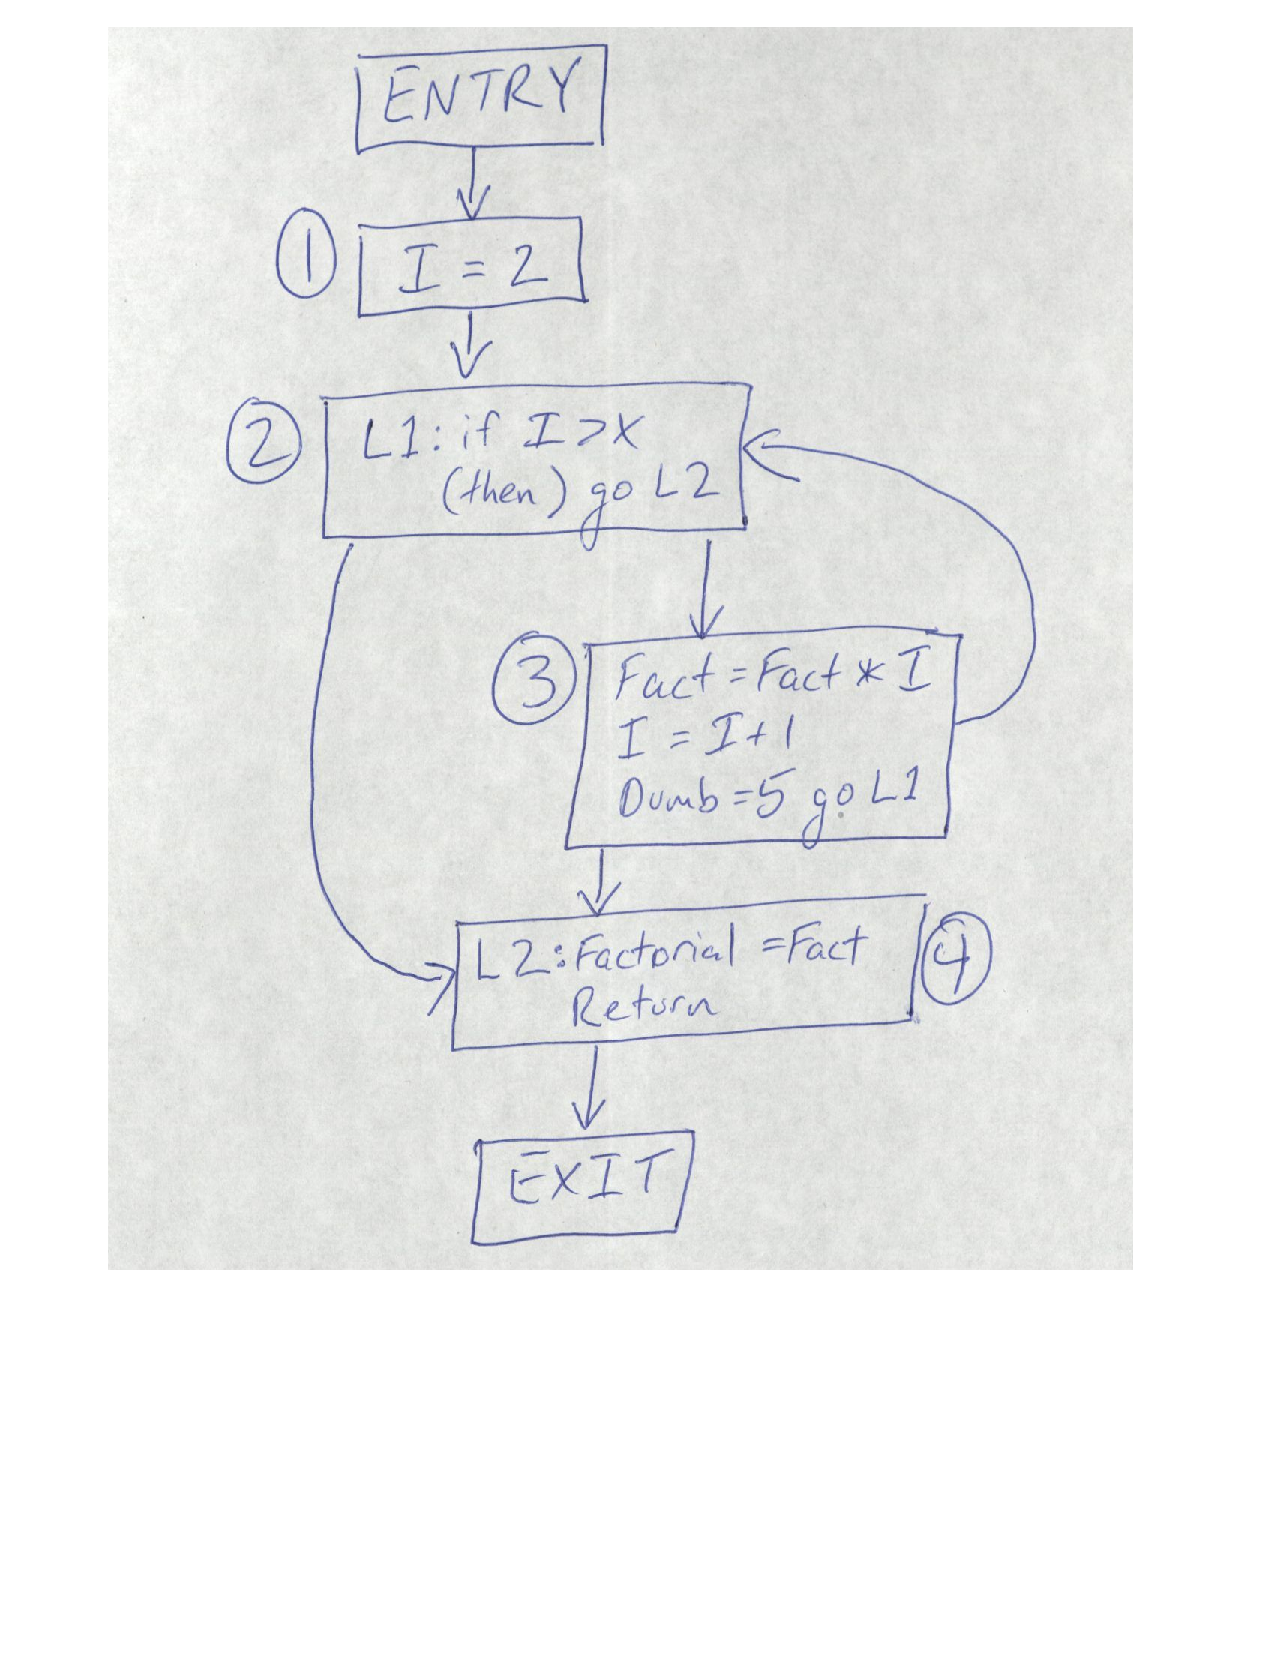
\includepdf[scale=0.25]{p1b.pdf}

\item 
\item 
\item 
\end{enumerate}

\item

\item

\end{enumerate}
\end{document}















